\subsubsection{Spiralmodell}
\label{sec:Kap-2.2.2.1}

\sttpLeserfuehrung{Bilder/Kapitel-2/Leserfuehrung/Vorgehensmodelle-2-2-2-Illustration.pdf}{Bilder/Kapitel-2/Leserfuehrung/Vorgehensmodelle-2-2-2-1.pdf}

Hauptziel des Spiralmodells ist das frühzeitige Erkennen von Entwicklungsrisiken (Scheitern des Projekts, Nichteinhalten von Zeit- und Kostenplänen, nicht umsetzbare Funktionalitäten etc.), um ihre Eintretenswahrscheinlichkeiten so weit wie möglich zu verringern. Der Fokus des Spiralmodells liegt daher auf Maßnahmen der Risikoanalyse und –vermeidung. Es trägt seinen Namen aufgrund einer spiralförmigen Darstellung, die darstellt, dass in jeder Iteration dieselben vier Segmente durchlaufen werden: 

\begin{enumerate}
	\item Bestimmung und Analyse von Zielen für die jeweilige Iteration
	\item Evaluierung von Lösungsmöglichkeiten, Bestimmung von Risiken und Maßnahmen zu deren Verringerung
	\item Realisierung von Lösungen (häufig durch Prototypen) und Bewertung der realisierten Lösung
	\item Planung der nächsten Iteration 
\end{enumerate}

\begin{figure}[h!]
    \centering
    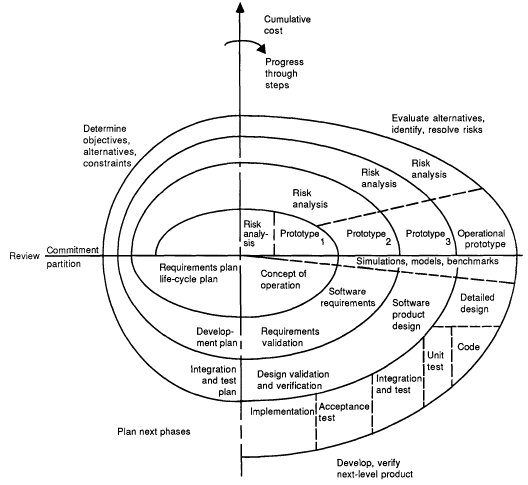
\includegraphics[scale=0.5]{Bilder/Kapitel-2/SpiralmodellBoehm.png}
    \caption{Spiralmodell von Boehm \cite[64]{boe88}}
    \label{fig:spiralmodell_von_boehm}
\end{figure}

Trotz der iterativen Elemente ist das Spiralmodell insofern auch sequentiell orientiert, als sich die ersten Iterationen schwerpunktmäßig mit der Definition der Anforderungen beschäftigen, die nächsten mit dem Systementwurf, die folgenden mit der Implementierung etc. Innerhalb einer einzelnen Iteration bleibt das Spiralmodell allerdings bewusst flexibel. So kann das Spiralmodell heute genauso mit sequentiellen wie auch agilen Methoden eingesetzt werden. In Kombination mit der Fokussierung auf Maßnahmen der Risikovermeidung statt auf die Prozesse des Softwareengineering ist das Spiralmodell kein typisches projektbezogenes Vorgehensmodell, sondern eher ein Metamodell, in dessen Rahmen Methoden verschiedener Vorgehensmodelle eingesetzt werden können. Aus heutiger Sicht liegt die Bedeutung des Spiralmodells vor allem darin, dass es schon in den 1980er Jahren – und damit zur Hochzeit der phasenorientierten Modelle – ein iteratives Vorgehen und den Einsatz von Prototypen für die Entwicklung eines Softwareprodukts propagierte. Zusammenfassende Darstellungen des Spiralmodells finden sich in \cite[556 \psqq]{bal08} und \cite[91  \psqq]{bro13}. Die Originalartikel von Barry W. Boehm zum Spi\-ral\-mo\-dell sind \cite{boe86} und \cite{boe88}.